\chapter{Evaluation Scenarios}%
\label{ch:evaluationscenarios}%


In this chapter, we present the scenarios used in the evaluation of this thesis.
We do not perform \emph{case studies} as we do not study the use of our contributions in a real-life environment, e.g., by watching software architects or security experts \cite{wohlin_case_2021}.
We use the term \emph{evaluation scenario} instead as we only investigate the intended use of our contributions based on real-world systems, similar to related work \cite{runeson_guidelines_2009,walter_context-based_2023}.
Nevertheless, using case study systems in the evaluation of contributions in the software architecture community is common \cite{walter_context-based_2023,seifermann_architectural_2022,busch_architecture-based_2020}.
\textcite{konersmann_evaluation_2022} conducted a \acf{SLR} with 153 papers and found that using case study systems represents the most common evaluation method in recent software architecture research.

In this thesis, every \emph{evaluation scenario} is based on or related to a real software system that has been specified by others.
Thus, we start each scenario with a description of its source, where it is used, and how the architectural models have been created.
Afterward, we describe the software system of each scenario, which includes the software architecture and its intended use.
Every scenario handles confidential data and thus has confidentiality requirements that can be specified as data flow constraints.
Last, a real-world software system is subject to uncertainty.
We discuss uncertainty sources and their potential impact on confidentiality based on existing collections \cite{hahner_classification_2023,ramirez_taxonomy_2012,hahner_arcn_2024}.

This chapter introduces six evaluation scenarios.
The first three, namely the \emph{TravelPlanner}, \emph{DistanceTracker}, and \emph{OnlineShop} scenarios have been used in the evaluation of related approaches \cite{walter_context-based_2023,seifermann_architectural_2022,seifermann_detecting_2022,seifermann_data-driven_2019,kunz_efficient_2018,weimann_automated_2017,walter_architectural_2022-1,walter_architecture-based_2023,walter_tool-based_2023,kramer_model-driven_2017}.
The second three, namely the \emph{CoronaWarnApp}, \emph{MobilityAsAService}, and \emph{JPlag}, represent software systems from academia \cite{leinweber_leveraging_2023,prechelt_finding_2002,saglam_automated_2024,saglam_detecting_2024,saglam_obfuscation-resilient_2024,saglam_token-based_2022} and industry \cite{robert_koch_institute_open-source_2020,enaya_case_2024}.
In the following, we give an overview of the evaluation scenarios and then introduce them in more detail.
See the data set \cite{dataset} for all data flow constraints and \acf{PCM} instances.

\ownpublications{
\fancycite{hahner_architectural_2021}, 
\fancycite{boltz_handling_2022},
\fancycite{walter_architectural_2022},
\fancycite{hahner_model-based_2023},\linebreak
\fancycite{hahner_classification_2023},
\fancycite{hahner_architecture-based_2023},
\fancycite{boltz_extensible_2024},\linebreak
\fancycite{hahner_arcn_2024}
}





\section{Overview}%
\label{sec:evaluationscenarios:overview}

\begin{table}
    \begin{tabularx}{\linewidth}{lllX}
        \toprule
        Name & Domain & Origin & Used in \\
        \midrule
        TravelPlanner & Mobility & \cite{katkalov_model-driven_2013,katkalov_modellgetriebener_2017} & \cite{walter_context-based_2023,seifermann_architectural_2022,seifermann_detecting_2022,seifermann_data-driven_2019,walter_architectural_2022-1,walter_architecture-based_2023,walter_tool-based_2023,kramer_model-driven_2017,hahner_model-based_2023,hahner_modeling_2021,walter_architectural_2022,boltz_handling_2022,schwickerath_tool-supported_2023} \\
        DistanceTracker & Health / Sports & \cite{katkalov_modellgetriebener_2017} & \cite{seifermann_architectural_2022,seifermann_detecting_2022,seifermann_data-driven_2019,hahner_model-based_2023,hahner_modeling_2021,walter_architectural_2022,boltz_handling_2022}  \\
        OnlineShop & E-Commerce & \cite{seifermann_data-driven_2019,rausch_common_2008} & \cite{walter_architectural_2022,kunz_efficient_2018,weimann_automated_2017,hahner_domain-specific_2020,hahner_model-based_2023,boltz_extensible_2024,hahner_architectural_2021,hahner_arcn_2024,hahner_classification_2023,hahner_architecture-based_2023} \\
        CoronaWarnApp & Health & \cite{robert_koch_institute_open-source_2020,enaya_case_2024} & \cite{hahner_classification_2023,hahner_architecture-based_2023,hahner_architecture-based_2024} \\
        MobilityAsAService & Mobility & \cite{leinweber_leveraging_2023} & - \\
        JPlag & Plagiarism Detection & \cite{prechelt_finding_2002,saglam_obfuscation-resilient_2024} & - \\
        \bottomrule
    \end{tabularx}
    \caption{Overview of all evaluation scenarios, their domain, their origin, and their usage.}%
    \label{table:evaluationscenarios:overview}
\end{table}

For the evaluation of this thesis, we use software systems and scenarios of different size and from different domains.
\autoref{table:evaluationscenarios:overview} shows an overview of the six evaluation scenarios, their origin, and other evaluations where they have already been used.
To encounter threats to external validity and to increase generalizability, we use scenarios from different domains, e.g., from the mobility or health domain.
All evaluation scenarios originate from other work.
The majority have been used in the evaluation of other publications.
Only the last two scenarios, \emph{MobilityAsAService} a service and \emph{JPlag} are new.
However, they represent well-evaluated systems with high demands on the systems' confidentiality and are thus suitable as evaluation scenarios for this thesis.

\begin{table}
    \begin{tabularx}{\linewidth}{lZZZZZZ}
        \toprule
        Name & \rot{\# Component} & \rot{\# \ac{SEFF}} & \rot{\# \ac{TFG}} & \rot{\# Vertex} & \rot{\# Uncertainty} & \rot{\# Violation} \\
        \midrule
        TravelPlanner & 7 & 9 & 2 & 42 & 1 & 1 \\
        DistanceTracker & 8 & 10 & 1 & 29 & 1 & 1 \\
        OnlineShop & 2 & 6 & 3 & 44 & 4 & 24 \\
        CoronaWarnApp & 21 & 58 & 14 & 687 & 9 & 163 \\
        MobilityAsAService & 18 & 49 & 8 & 200 & 5 & 6 \\
        JPlag & 3 & 5 & 3 & 65 & 4 & 26 \\
        \bottomrule
    \end{tabularx}
    \caption{Size metrics, uncertainty sources, and confidentiality violations of all evaluation scenarios.}%
    \label{table:evaluationscenarios:size}
\end{table}

For the contributions of this thesis (\C{1}, \C{2}, and \C{3}), a central property of a software system is the form and size of the system's \acf{DFD} and the scenario's uncertainty sources, as discussed in \autoref{sec:classification:dfd} and \autoref{sec:confidentialityanalysis:typeagnostic}.
\autoref{table:evaluationscenarios:size} lists all relevant size-related metrics of the six evaluation scenarios.
This includes the number of the components and \acfp{SEFF} of the \ac{PCM} instance of each scenario, as these numbers impact the number of \ac{DFD} nodes.
We also show the number of \acfp{TFG} and their vertices, because these sizes are relevant both for the uncertainty impact analysis (\C{2}) and for the different approaches to uncertainty-aware data flow analysis (\C{3}).
Last, we show the number of uncertainty sources in the evaluation scenarios and the number of potential confidentiality violations due to these uncertainties.

The scenarios show different sizes and numbers of uncertainties and violations. The \emph{TravelPlanner} and the \emph{DistanceTracker} represent smaller scenarios with one uncertainty source each, and 7 and 8 components, respectively.
Still, their \acp{TFG} have a total of 42 and 29 vertices, which highlights again the need for automated analysis approaches and tool support, discussed in \autoref{sec:overview:toolsupport}.
\emph{MobilityAsAService} and \emph{CoronaWarnApp} are the largest evaluation scenarios.
They contain 5 and 9 uncertainty sources and a total of 200 and 687 \ac{TFG} vertices that represent \ac{DFD} nodes.





\section{TravelPlanner}%
\label{sec:evaluationscenarios:travelplanner}

\begin{figure}
    \centering
    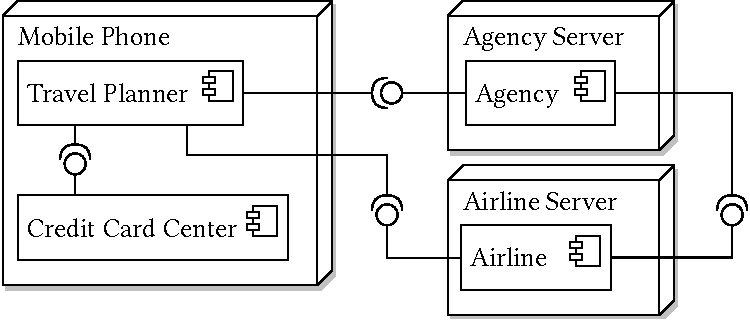
\includegraphics[width=0.7\textwidth]{figures/chapter8/scenario1_travelplanner.pdf}
    \caption{Simplified component and deployment diagram of the TravelPlanner evaluation scenario.}
    \label{fig:evaluationscenarios:travelplanner}
\end{figure}

\paragraph{Source}
The \emph{TravelPlanner} evaluation scenario originates from the iFlow project by \textcite{katkalov_modellgetriebener_2017}.
It originally has been used in the evaluation of information flow analysis \cite{katkalov_model-driven_2013}.
A comprehensive description of the software architecture and a Java-based implementation are available \cite{katkalov_modeling_2013}.
The \ac{PCM} model used in this evaluation scenario stems from related work \cite{seifermann_architectural_2022,walter_context-based_2023} and has been used in many case study-based validations \cite{seifermann_detecting_2022,seifermann_data-driven_2019,walter_architectural_2022-1,walter_architecture-based_2023,walter_tool-based_2023,kramer_model-driven_2017,hahner_model-based_2023,hahner_modeling_2021,walter_architectural_2022,boltz_handling_2022,schwickerath_tool-supported_2023}.

\paragraph{Description}
\autoref{fig:evaluationscenarios:travelplanner} shows a simplified diagram of the software architecture.
Here---and also in all following figures of this chapter---we show simplified diagrams to give an overview and to increase clarity.
As shown in \autoref{table:evaluationscenarios:size}, the \ac{PCM} model consists of more components than illustrated.
We do also not depict uncertainty sources in this diagram.
We refer to the data set \cite{dataset} for the complete architectural model, which includes data flow constraints and uncertainty models.
The corresponding \ac{PCM} model consists of 7 components with 9 \acp{SEFF} and maps to 2 \acp{TFG} with 42 vertices.

This evaluation scenario comprises three central entities: A customer, a travel agency, and an airline.
The customer uses the \emph{Travel Planner} app to search for flights.
This app communicates with a travel \emph{Agency} that queries flights from multiple \emph{Airlines}.
The aggregated results are returned to the customer.
Afterward, the customer selects and books a flight using a credit card.
The software architecture comprises three deployment locations that match the three entities.
The customer operates the \emph{Mobile Phone}, where the \emph{Travel Planner} app and the \emph{Credit Card Center} app is located.
Both the \emph{Agency} and the \emph{Airline} operate their own servers and provide interfaces to the other components.

\paragraph{Confidentiality requirements}
In this evaluation scenario, we consider two different data types.
On the one hand, the flight data represents public information without any data flow constraints.
On the other hand, credit card data represents highly sensitive information with strict confidentiality requirements.
This information is managed by the \emph{Credit Card Center} and shall only leave the \emph{Mobile Phone} in the booking process upon explicit approval by the customer.
Additionally, the credit card data shall only flow directly to the \emph{Airline} in the booking process---it shall never flow to the \emph{Agency}.

\paragraph{Uncertainty sources}
We use this evaluation scenario as a minimal scenario for \emph{primary} uncertainty.
We add the \emph{Behavior} uncertainty that credit card data can be used with or without user consent \cite{hahner_model-based_2023}.
Here, passing the data to the \emph{Airline} servers without consent represents a violation of the aforementioned confidentiality requirements.





\section{DistanceTracker}%
\label{sec:evaluationscenarios:distancetracker}

\begin{figure}
    \centering
    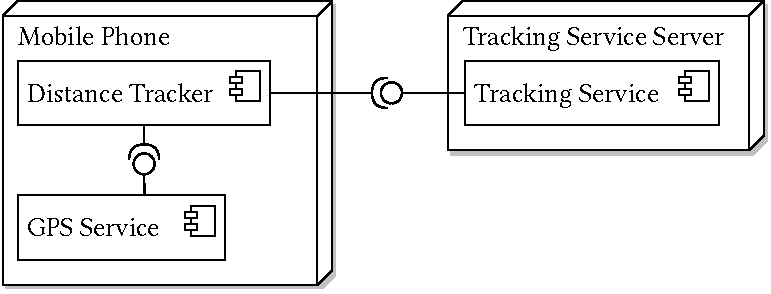
\includegraphics[width=0.7\textwidth]{figures/chapter8/scenario2_distancetracker.pdf}
    \caption{Simplified component and deployment diagram of the DistanceTracker evaluation scenario.}
    \label{fig:evaluationscenarios:distancetracker}
\end{figure}

\paragraph{Source}
The \emph{DistanceTracker} evaluation scenario also originates from the iFlow project by \textcite{katkalov_modellgetriebener_2017}.
Similarly to the \emph{TravelPlanner} scenario described above, it has been used in many case study-based validations \cite{seifermann_architectural_2022,seifermann_detecting_2022,seifermann_data-driven_2019,hahner_model-based_2023,hahner_modeling_2021,walter_architectural_2022,boltz_handling_2022}.

\paragraph{Description}
\autoref{fig:evaluationscenarios:distancetracker} shows a simplified diagram of the software architecture.
As discussed above, we simplify the system structure and do not depict uncertainty sources to increase clarity and refer to the data set \cite{dataset}.
The corresponding \ac{PCM} model consists of 8 components with 10 \acp{SEFF} and maps to 1 \ac{TFG} with 29 vertices.

The evaluation scenario comprises three central entities: The user, the \emph{Distance Tracker} app, and the online \emph{Tracking Service}.
The user shares the GPS location with the tracking app that periodically tracks the current location and calculates the distance run.
This distance is transmitted to the \emph{Tracking Service}.
The software architecture comprises two deployment locations.
The user operates the \emph{Mobile Phone} that hosts the \emph{Distance Tracker} app and a \emph{GPS service}.
The \emph{Tracking Service} is deployed on a separate server.

\paragraph{Confidentiality requirements}
The confidentiality requirement of this evaluation scenario considers the confidentiality of GPS data, i.e., precise information about the user's current location.
This information is only allowed to be used locally on the \emph{Mobile Phone}.
Only in aggregated form, e.g., as calculated distance, this information is allowed to be passed to the \emph{Tracking Service}.
Thus, there shall be no flow of explicit GPS locations from the \emph{Mobile Phone} to any other location.

\paragraph{Uncertainty sources}
We use this evaluation scenario as a minimal scenario for \emph{secondary} uncertainty.
We add the \emph{Connector} uncertainty that GPS data can be processed on the \emph{Tracking Service Server} \cite{hahner_model-based_2023} for additional statistics and a persisted history of runs.
Passing the GPS data to the \emph{Tracking Service} for this purpose is a confidentiality violation.





\section{OnlineShop}%
\label{sec:evaluationscenarios:onlineshop}

\begin{figure}
    \centering
    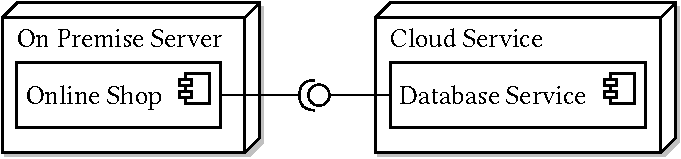
\includegraphics[width=0.65\textwidth]{figures/chapter8/scenario3_onlineshop.pdf}
    \caption{Simplified component and deployment diagram of the OnlineShop evaluation scenario.}
    \label{fig:evaluationscenarios:onlineshop}
\end{figure}

\paragraph{Source} 
The \emph{OnlineShop} evaluation scenario is based on CoCoME \cite{rausch_common_2008} and has been adapted for architecture-based confidentiality analysis \cite{seifermann_data-driven_2019}.
It has also been used in case study-based validations \cite{walter_architectural_2022,kunz_efficient_2018,weimann_automated_2017,hahner_domain-specific_2020,hahner_model-based_2023,boltz_extensible_2024,hahner_architectural_2021,hahner_arcn_2024,hahner_classification_2023,hahner_architecture-based_2023}.
We refer to this evaluation scenario throughout this thesis as the running example\footnote{Although using an evaluation scenario as the running example represents a threat to validity, we argue that this threat is weakened by using other evaluation scenarios in addition. Furthermore, the increased understanding arising from such thorough investigation can benefit the evaluation.}, see \autoref{ch:runningexample}.

\paragraph{Description}
\autoref{fig:evaluationscenarios:onlineshop} shows a simplified diagram of the software architecture.
A comprehensive diagram of the software system is shown in \autoref{fig:runningexample:architecture}, and the architectural model is part of the data set \cite{dataset}. 
The corresponding \ac{PCM} model consists of 2 components with 6 \acp{SEFF} and maps to 3 \acp{TFG} with 44 vertices.

The evaluation scenario comprises three central entities: The customer, the \emph{Online Shop}, and the shop's \emph{Database Service}.
We consider three usage scenarios: The user can query available items, purchase items, and request a support contact.
The former two scenarios include calls of the \emph{Online Shop} to the \emph{Database Service}, the latter only yields static information.
The software architecture comprises two deployment locations.
The \emph{Online Shop} is deployed \emph{On Premise} while the \emph{Database Service} is deployed to a \emph{Cloud Service}.
We refer to \autoref{ch:runningexample} for a more detailed description of the software system.

\paragraph{Confidentiality requirements}
In this evaluation scenario, we consider two different data types.
The public information of the online shop, like available items, and the user's private purchase details.
While the former is publicly available and not sensitive, the latter is highly sensitive, comparable to the credit card details of the \emph{TravelPlanner} evaluation scenario.
The user input in the purchase process shall be validated and encrypted before flowing into the database.
Additionally, depending on the deployment location and the trustworthiness of the resource provider, confidentiality can be threatened.
We provide more details on the confidentiality requirements in \autoref{ch:runningexample}.

\paragraph{Uncertainty sources}
We define four uncertainty sources in this evaluation scenario, as described in \autoref{sec:runningexample:uncertainty}.
Uncertainty \U{1} affects the user input that can be valid, erroneous, or malicious.
Uncertainty \U{2} affects the data processing in the \emph{Online Shop} component that can validate or encrypt the data.
Uncertainty \U{3} affects the deployment of the \emph{Database Service} component that can be on-premise or in the cloud. 
Uncertainty \U{4} affects the trustworthiness of the provider of the \emph{Cloud Service} that can be trustworthy or suspicious.
All uncertainty sources and their scenarios are shown in \autoref{table:confidentialityanalysis:scenarios}.





\section{CoronaWarnApp}%
\label{sec:evaluationscenarios:coronawarnapp}

\begin{figure}
    \centering
    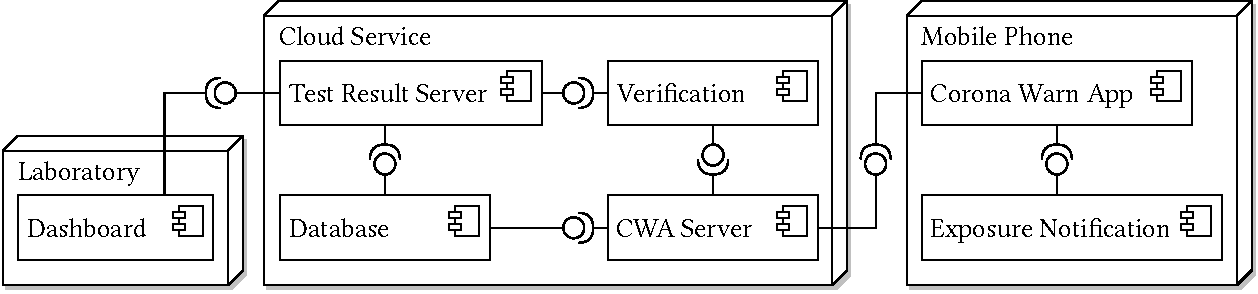
\includegraphics[width=\textwidth]{figures/chapter8/scenario4_coronawarnapp.pdf}
    \caption{Simplified component and deployment diagram of the CoronaWarnApp evaluation scenario.}
    \label{fig:evaluationscenarios:coronawarnapp}
\end{figure}

\paragraph{Source}
The \emph{CoronaWarnApp} evaluation scenario is based on the German Contact Tracing App of the same name \cite{robert_koch_institute_open-source_2020}.
During the COVID-19 pandemic, this app was used to warn users who may have come into contact with people who had tested positive on COVID-19.
The app was developed by SAP and Deutsche Telekom \cite{enaya_case_2024}, published by the Robert Koch Institute, and downloaded more than 20 million times \cite{robert_koch_institute_open-source_2020}.
All source code and documentation are available open-source on GitHub \cite{sap_corona-warn-app_2023}, including a detailed description of the software architecture.
We used the publicly available information to create a \ac{PCM} model that was already used in multiple validations \cite{hahner_classification_2023,hahner_architecture-based_2023,hahner_architecture-based_2024}.

\paragraph{Description}
\autoref{fig:evaluationscenarios:coronawarnapp} shows a simplified diagram of the software architecture.
Due to the size of the evaluation scenario, we leave out many details in this diagram, e.g., the collection of statistics, or the international exchange of positive test results.
The \ac{PCM} component repository model is shown in \autoref{sec:appendix:cwa}.
The corresponding \ac{PCM} model consists of 21 components with 58 \acp{SEFF} and maps to 14 \acp{TFG} with 687 vertices.

The evaluation scenario comprises five central entities.
The user of the app, the server infrastructure, laboratories, support hotlines, and international partners.
Users can voluntarily enter if they are infected to warn others and they also get warned in the case of a potential contact.
The warning mechanism uses keys that are exchanged between mobile phones via Bluetooth \cite{sap_corona-warn-app_2023}.
If users are tested, they can enter the test via a code or with the help of the support hotline.
The laboratories add the test results, and the server infrastructure manages both.
Additionally, the keys of positive tested users can be shared with international partner servers in the EU and Switzerland.
The components of the server infrastructure, e.g., the \emph{Verification}, or the \emph{Test Result Server}, are deployed to the \emph{Cloud Service} of the Open Telekom Cloud.
Laboratories operate their own \emph{Dashboards} and laboratory information systems that connect to the server infrastructure.
Users have the \emph{Corona Warn App} installed on their phones that communicate with the \emph{Exposure Notification} framework.
This framework manages the key exchange and comparison.

\paragraph{Confidentiality requirements}
The Corona Warn App manages sensitive information related to health data and location data.
Contact tracing apps are challenged with many risks, e.g., regarding de-anonymization or profiling \cite{baumgartner_mind_2020}.
We express multiple confidentiality requirements as data flow constraints \cite{hahner_modeling_2021,boltz_extensible_2024}.
First, users should not be able to directly access the exchanged keys but only be warned if an exchanged key matches a key of a person who tested positive.
Additionally, all keys and other credentials are considered to be sensitive information.
Here, the \emph{Verification} component plays a central role in the validation.
The Corona Warn App collects statistical data that shall only be shared in aggregated form.
Last, we reuse the already discussed requirements regarding secure storage, information leaks, and logging.
The full list of requirements is in data set \cite{dataset}.

\paragraph{Uncertainty sources}
Due to the size of this evaluation scenario, we model 4 sub-scenarios with 2 to 3 uncertainty sources each, which adds up to a total of 9 uncertainty sources.
In this first sub-scenario, we consider the processing of data and the interception of the communication regarding a central component in the \emph{Cloud Service}.
The second sub-scenario focuses on deployment and secure storage of test results using the \emph{Test Result Server}.
The third sub-scenario evolves around logging and validation in the \emph{Verification} component.
In the fourth sub-scenario, we focus on critical points within the system with a potentially wide impact, e.g., the \emph{Database} and the \emph{Exposure Notification} framework.
All details about the uncertainty sources and scenarios can be found in the data set \cite{dataset}.





\section{MobilityAsAService}%
\label{sec:evaluationscenarios:mobilityasaservice}

\begin{figure}
    \centering
    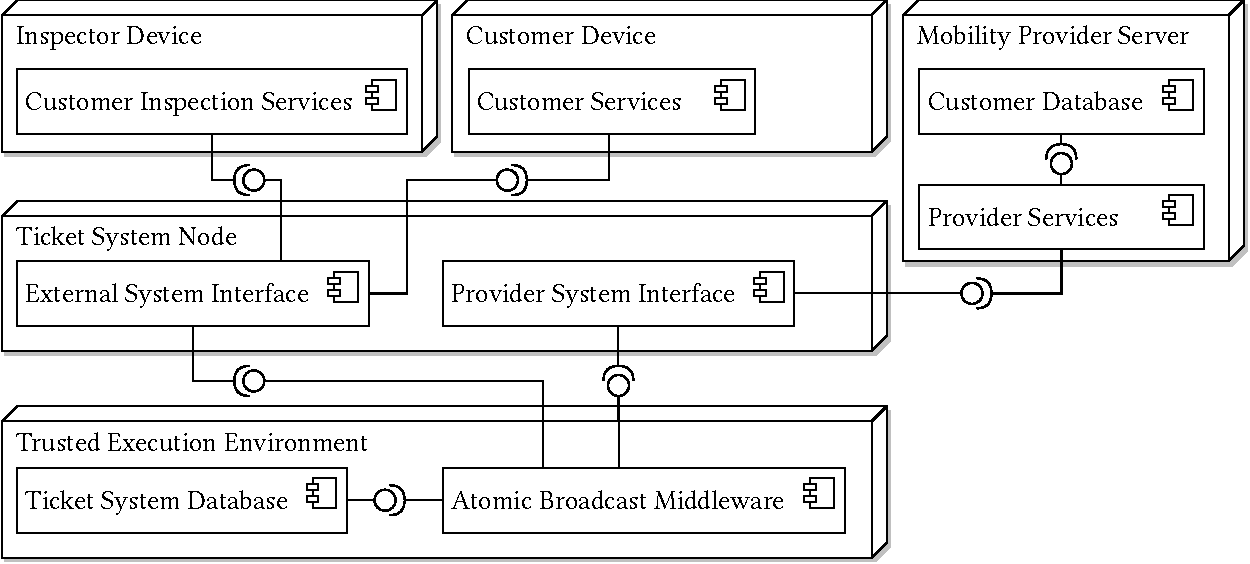
\includegraphics[width=\textwidth]{figures/chapter8/scenario5_mobilityasaservice.pdf}
    \caption{Simplified component and deployment diagram of the MobilityAsAService evaluation scenario.}
    \label{fig:evaluationscenarios:mobilityasaservice}
\end{figure}

\paragraph{Source}
The \emph{MobilityAsAService} evaluation scenario is based on a concept for a distributed ticketing system of the same name \cite{leinweber_leveraging_2023}.
It uses \acf{DLT} with \acfp{TEE} to define a secure system with distributed governance that is scalable while ensuring confidentiality.
We used the available documentation to create a \ac{PCM} model that approximates the proposed concept.

\paragraph{Description}
\autoref{fig:evaluationscenarios:mobilityasaservice} shows a simplified diagram of the software architecture.
As we use the \ac{ADL} \ac{PCM} to model the scenario, we can only approximate the actual behavior of a \ac{DLT}, or a \ac{TEE}.
Additionally, we only model one mobility provider, while the underlying concept allows for many operators with decentralized governance. 
The corresponding \ac{PCM} model consists of 18 components with 49 \acp{SEFF} and maps to 8 \acp{TFG} with 200 vertices.

The evaluation scenario comprises four central entities.
The ticket system encapsulates a \ac{TEE} that manages a replicated state machine and middleware to broadcast requests.
We illustrate this with the \emph{Ticket System Database} and the \emph{Atomic Broadcast Middleware} components.
The system can receive input from the three other entities: Inspectors, customers, and mobility providers.
Each node provides an \emph{External System Interface} for the former two and a \emph{Provider System Interface} for the latter.
Customers can register, check-in, check-out, and see their trip history through several components that we bundled as \emph{Customer Services}.
Inspectors can inspect customers using the \emph{Customer Inspection Services}, i.e., check the current state of the customer.
Mobility Providers have tools for billing, clearance, and analysis as part of the \emph{Provider Services}.
Additionally, they store contact and billing information of their customers in a separate \emph{Customer Database}.
We combined some of the aforementioned services, e.g., the \emph{Customer Services}, for the sake of clarity, the full model is part of the data set \cite{dataset}.

\paragraph{Confidentiality requirements}
\textcite{leinweber_leveraging_2023} name several confidentiality requirements of the \emph{MobilityAsAService} system.
They require that only authorized entities are able to access the data of the ticket system.
Additionally, providers' business secrets and customer data shall not be leaked during the replication process.
Details about individual trips shall not be revealed to providers who only see the total invoice value.
The system is designed to provide all entities with the minimal information required for their tasks.

\paragraph{Uncertainty sources}
We use this evaluation scenario to combine all five types of uncertainty sources defined in \autoref{table:classification:classification:architecturalelementtype}.
We add an \emph{External} uncertainty to a staff member who uses the \emph{Provider Services} regarding the member's role and authorization.
We add a \emph{Behavior} uncertainty to the \emph{Ticket System Database} regarding the granularity of the retrieved data.
We add a \emph{Interface} uncertainty to the trip history service that is part of the \emph{Customer Services}, and a \emph{Connector} uncertainty to the customer registration that is part of the \emph{Customer Services}, both regarding the sensitivity of the retrieved data.
Last, we add a \emph{Component} uncertainty to the \emph{Provider Services} representing a malicious mobility provider \cite{leinweber_leveraging_2023}.
All uncertainty sources reflect changes to the \emph{MobilityAsAService} concept that would violate confidentiality.





\section{JPlag}%
\label{sec:evaluationscenarios:jplag}

\begin{figure}
    \centering
    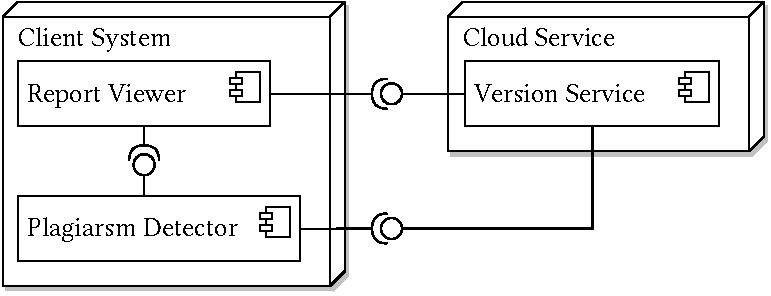
\includegraphics[width=0.7\textwidth]{figures/chapter8/scenario6_jplag.pdf}
    \caption{Simplified component and deployment diagram of the JPlag evaluation scenario.}
    \label{fig:evaluationscenarios:jplag}
\end{figure}

\paragraph{Source}
The \emph{JPlag} evaluation scenario is based on the plagiarism detector of the same name \cite{prechelt_finding_2002}.
Plagiarism detectors compare models or code submissions of programming tasks \cite{saglam_token-based_2022}, e.g., in educational context \cite{saglam_how_2023}, to find suspicious similarities, i.e., plagiarism \cite{saglam_obfuscation-resilient_2024}.
The \emph{JPlag} project, started in 1996, represents one of the most widely-used plagiarism detectors that is resilient against most obfuscation attempts \cite{saglam_obfuscation-resilient_2024,saglam_automated_2024,saglam_detecting_2024,saglam_jplag_2024,saglam_mitigating_2025,schmid_jplag_2025}.
Since 2020, the software architecture of \emph{JPlag} has been re-engineered.
Based on the available documentation of this open-source project \cite{saglam_jplag_2024}, and by cooperating with the current maintainers, we created a \ac{PCM} model of the core functionality.

\paragraph{Description}
\autoref{fig:evaluationscenarios:jplag} shows a simplified diagram of the software architecture.
The \emph{Jplag} software architecture is designed to enable the deployment of the main components, i.e., the \emph{Plagiarism Detector} and the \emph{Report Viewer}, on a client system, a local machine, or a server, to simplify its integration into other products \cite{saglam_jplag_2024}.
Nevertheless, we consider the illustrated deployment to be the most common use case.
The corresponding \ac{PCM} model consists of 3 components with 5 \acp{SEFF} and maps to 3 \acp{TFG} with 65 vertices.

The evaluation scenario comprises three entities: The \emph{Plagiarism Detector}, a \emph{Report Viewer} for displaying analysis results, and a \emph{Version Service} for update notifications.
The \emph{Plagiarism Detector} receives a set of code or model submissions as input and compares them.
This is done internally without any communication to other services \cite{saglam_jplag_2024}.
After the comparison, all results are stored in an archive.
This includes similarity scores between submissions, clusters of similar submissions, or suspiciously similar parts of the submissions.
Because plagiarism detection needs human judgment \cite{saglam_obfuscation-resilient_2024,saglam_detecting_2024}, the results are displayed in a human-readable way using the \emph{Report Viewer}.
The software architecture supports the direct communication between the \emph{Plagiarism Detector} and the \emph{Report Viewer}, but users can also choose to manually load a result archive, e.g., to revisit older comparisons.
The \emph{Report Viewer} is web-based but only operates within the web browser without the need for additional server infrastructure \cite{saglam_jplag_2024}.
Thus, all input remains on the users' \emph{Client System}.
As \emph{Jplag} is subject to continuous development \cite{saglam_jplag_2024}, both components communicate with a \emph{Version Service} to notify users about available updates.

\paragraph{Confidentiality requirements}
Plagiarism detectors like \emph{JPlag} are designed for the educational context, e.g., programming tasks.
Here, student data has to be treated as confidential due to administrative rules and laws like the \acf{GDPR} \cite{council_of_european_union_regulation_2016}.
We interpret this requirement as data flow constraint and restrict that all submissions and all plagiarism detection results shall never leave the client system.
Furthermore, the authors of \emph{JPlag} claim to never collect any usage data from running the software \cite{saglam_jplag_2024}.
Thus, we additionally restrict the \emph{Version Service} to not collect or evaluate any statistical information on the versions in use.

\paragraph{Uncertainty sources}
We use this evaluation scenario to define four uncertainty sources, of which only two negatively affect the system's confidentiality.
This allows for more precise statements about potential false positives in the evaluation \cite{powers_evaluation_2011}.
The first uncertainty source considers the deployment of the \emph{Report Viewer} on the \emph{Client System} or in the cloud.
The second uncertainty source considers the usage of \emph{JPlag} standalone or in conjunction with the \emph{Report Viewer}.
As stated previously, neither uncertainty affects the confidentiality of the software architecture.
The third uncertainty source targets the deployment of the \emph{Plagiarism Detector}, which could be deployed locally or in the cloud.
This could cause sensitive student data to flow to another server, which violates confidentiality---an argument against closed-source plagiarism detection as a service \cite{saglam_obfuscation-resilient_2024,saglam_jplag_2024}.
Last, we add a fourth uncertainty concerning the data collection behavior of the \emph{Version Service}.
As stated previously, evaluating usage data violates confidentiality.





\section{Summary and Outlook}%
\label{sec:evaluationscenarios:summary}

In this chapter, we presented six evaluation scenarios that will be used throughout the evaluation of this thesis.
All evaluation scenarios are based on or related to a case study of a software system that handles confidential data.
The scenarios have different sizes that range from 2 to 21 components, and also have different origins and domains.
For each evaluation scenario, we described its source, software architecture, confidentiality requirements, and uncertainty sources.
All scenarios are modeled using the \ac{PCM}.

The first scenario, the \emph{TravelPlanner}, represents a smartphone app to search and book flights.
The second scenario, the \emph{DistanceTracker}, is a sports or health app that tracks the distance run by a user.
The third scenario, the \emph{OnlineShop}, is an e-commerce application for purchasing items online, introduced in \autoref{ch:runningexample}.
The fourth scenario, the \emph{CoronaWarnApp}, is a contact tracing app developed during the COVID-19 pandemic.
The fifth scenario, \emph{MobilityAsAService}, is a distributed ticketing system based on \ac{DLT} and \acp{TEE}.
The sixth scenario, \emph{JPlag}, is a plagiarism detector, e.g., used for programming tasks in universities.

In sum, these scenarios provide a wide range of different software systems.
Despite their differences in structure and size, they all have to ensure the confidentiality of the processed data.
Furthermore, they are all subject to uncertainty.
We use these scenarios throughout \readingpath{ch:evaluation}.
For more details on the third scenario, the \emph{OnlineShop}, see \readingpath{ch:runningexample}.
For a more detailed view of the components of the fourth scenario, the \emph{CoronaWarnApp}, see \autoref{sec:appendix:cwa}.
Last, we again refer to our data set \cite{dataset} for all uncertainty and architectural models and all data flow constraints.





\section{In Simpler Words}%
\label{sec:evaluationscenarios:simple}

In the last three chapters, we presented the contributions of this thesis.
In our research area, a contribution is an enhancement of the state of the art, e.g., a new or better algorithm, a better way to collect and express knowledge, or a new method.
To investigate the quality of our contributions, we perform an evaluation.
In the discipline of this thesis---software architecture research---many evaluations are based on case studies.
In this chapter, we refer to evaluation scenarios comparable to case studies.

We present six different evaluation scenarios of different sizes and from different domains.
Examples are the health domain, the mobility domain, and e-commerce.
Many of our evaluation scenarios have already been used to evaluate related approaches, e.g., the \emph{TravelPlanner} evaluation scenario.
Other scenarios, e.g., the \emph{CoronaWarnApp} evaluation scenario, are newer but based on well-studied software systems from the real world.
It is important to cover different sizes and domains because otherwise, one could say: \enquote{Your contributions only work for small software systems} or \enquote{Your contributions only work for systems in the mobility domain, but not for others}.
By using various evaluation scenarios, we counteract such---otherwise justified---criticism.
The following chapter will apply our contributions to these evaluation scenarios.
